\documentclass[10pt,conference]{IEEEtran}
% \IEEEoverridecommandlockouts

\usepackage{cite}
\usepackage{times}
\usepackage{url}
\usepackage[hidelinks]{hyperref}
\usepackage{hypernat}
\usepackage{graphicx}
\usepackage{listings}

\lstset{
  basicstyle=\footnotesize\ttfamily,
  commentstyle=\ttfamily,
  showstringspaces=false,
  xleftmargin=\parindent,
  numbers=left
}

\begin{document}

\title{Parallel Debugger}

\author{
  Luthra Milind Vikas 150363 \and
  Subhdeep Saha 150732
}

\maketitle

\section{Problem Statement}

While there are a plethora of debuggers for serial code - every IDE has one, and of course there is \texttt{gdb} - it is quite hard to debug parallel code, especially at the student level, and we are forced to use inelegant mechanisms like inserting \texttt{printf} functions in our code and re-running them. Our project focuses on making an open-source parallel debugger well-suited to educational purposes.

\section{Previous Work}

There are several existing debugging methods that can be used for debugging MPI based programs.

\subsection{Commercial Alternatives}

There are two commercially developed programs that facilitate parallel debugging, Arm DDT (Allinea DDT) \cite{ddt} and TotalView for HPC \cite{totalview}. Both of these tools are feature rich, working for not just MPI but also OpenMP, CUDA etc, and having support for basic Linux systems to supercomputers. These provide pretty GUI tools for visualization as well.

However, these tools are very expensive. Allinea DDT costs around \$600 for one licence which is further limited to a certain number of processes, and TotalView does not even list a cost outright, only the company can be contacted for evaluation of the software. Both these are targeted towards enterprise/large-scale users, and not those who are learning parallel computing. Further, both these tools are closed source, which limits access to their source code, and we cannot modify it as per our needs.

\subsection{Using xterm and gdb}

Another way to debug is to run all your processes inside \texttt{gdb} and then open all of them inside different \texttt{xterm} instances \cite{openmpidebug}, and then debug them each individually. This strategy does not scale to more than a handful of processes, because it is very tedious to keep changing terminals while trying to debug. In certain cases, this will not even work for processes distributed amongst nodes.

Clearly, this is too limited to be of any use once any serious debugging is needed.

\section{Overall Project Idea}

Our idea is based on the idea given above in \cite{openmpidebug}, through multiple \texttt{gdb} instances. However, instead of forcing the user to manually deal with each of the processes, we use a centralized server that connects to and orchestrates each process. The server does additional bookkeeping as well, to track some common errors that users are often prone to making.

The project is written almost entirely in Go, and communication between processes and the server is through TCP sockets. An overview of the project in Fig \ref{fig:overview} describes the various roles that will be discussed in detail in Section \ref{sec:impl}



\section{Features}

There are three main features of the project, whose implementation is discussed in detail later.

\begin{itemize}
\item \textbf{Client-Server Orchestration}: Our code instruments the target process, connects the client/server together, and makes possible controlling remotely the gdb instances. Commands can be sent to all or specific rank(s).
\item \textbf{TUI}: We provide a terminal-based user interface, suitable for use on the CSE cluster. We group outputs by the ranks.
\item \textbf{Collective Tracking}: Our code does some book-keeping to track collective calls, and find out which calls are pending at which ranks. This is useful for detecting common errors where the call to some collective is missing.
\end{itemize}

\section{Implementation Details}
\label{sec:impl}

\subsection{gdb/mi Interface}

\texttt{gdb/mi} is a machine-readable interface to the debugger. As opposed to the usual back and forth interaction that one has with the CLI, this can be thought of as two distinct streams: one in which we can write the input commands to be run, and the other an output stream, which runs asynchronously.

For example, calling \texttt{continue} in the CLI interface will cause the program to run (blocking any other commands) till a breakpoint is hit or the program ends. In MI interface, calling the equivalent of \texttt{continue} will return immediately, and tell us that the program is running. A stop notification is generated distinct to the \texttt{continue} call.

There is a Go library \cite{gogdb} which allows us to interact with the MI interface. We used that with a slight modification \cite{gogdbm}, to allow for commands in the usual CLI format as well as the MI format that the library permits.

The file of interest is \texttt{gdb.go}. Here, we will highlight a few things. First, how we have implemented a synchronous (blocking) method to send commands - it involves two functions, \texttt{SynchronizedSend} and \texttt{handleNotifications}. The first function is the exposed API for the \texttt{GDBInstance} object, while the second is an event handler that is automatically called by the \texttt{gdb} library when an asynchronous notification is received.

\begin{samepage}
\begin{lstlisting}[language=Go, caption=Partial pseudocode for Synchronized Send]
  func handleNotification(notification) {
    switch notification["class"] {
      case "running":
        bkptHitNotification.wait()
      case "stopped":
        bkptHitNotification.notify()
      }
   }

   func SynchronizedSend(message) {
     result = internalSend(message)
     handleNotification(result)
   }
\end{lstlisting}
\end{samepage}
In explanation, consider the following sequence:

\begin{itemize}
  \item We run a command like \texttt{continue}.
  \item \texttt{internalSend} returns a result - of the same type as a notification, with
    the class as running. We call \texttt{handleNotifications} and the thread waits on \texttt{bkptHitNotification}.
  \item When \texttt{continue} eventually runs and the program stops again, we get a notification again, with the class stopped. Then, the \texttt{bkptHitNotification} is notified, and the whole command is thus synchronized.
\end{itemize}

The second thing to be highlighted is the presence of hooks. An example of a hook can be found in \texttt{pd-client/main.go:51}, where the console output is sent to the server so that it can be echoed for the user.

\begin{samepage}
  \begin{lstlisting}[language=Go, caption=Custom hooks for notifications]
...
gdbInstance.AddNotificationHook(
func(notification) {
  if notification["type"]=="console" {
    // On getting a console notification,
    // relay it to the server.
    sendToServer(payload)
  }
  return true
})
...
\end{lstlisting}
\end{samepage}

\subsection{Start-up Instrumentation}

Starting up involves the connection of the server with all the clients, and the server needs to know the rank of each of the process running inside each of the clients as well.

As soon as the \texttt{pd-client} starts up, it connects to a \texttt{pd-server} (the host/port are command line arguments) and starts up an instance of \texttt{gdb}. Then, the target binary is loaded into this debugger instance. While loading the binary, we make use of \texttt{LD\_PRELOAD}. We have a shared library distributed with the client, which provides an implementation for \texttt{MPI\_Init}. This custom implementation calls \texttt{PMPI\_Init}, and then writes the rank of the process and the size of the WORLD communicator to a file.

\begin{samepage}
  \begin{lstlisting}[language=C, caption=Start-up instrumentation]
    int MPI_Init(int *argc, char ***argv) {
      ...
      return_code = PMPI_Init(argc, argv);
      MPI_Comm_rank(MPI_COMM_WORLD, &rank);
      MPI_Comm_size(MPI_COMM_WORLD, &size);
      write_to_file(filename, rank, size)
      return return_code;
    }
  \end{lstlisting}
\end{samepage}

We insert a breakpoint at the end of this function using \texttt{gdb}, and run the program. We access the file written by the custom implementation inside Go code to extract rank/size information and send to the server. When all of the processes have completed these steps, then the start-up is complete.

\begin{samepage}
  \begin{lstlisting}[language=Go, caption=gdb.go: InitGdb]
func InitGdb(debugTarget string) {
  ...
  SynchronizedSend("file", targetBinaryFilename)
  // Set up gdb environment containing LD_PRELOAD
  // and random filename FILENAME.
  SynchronizedSend("break PMPI_Init")
  SynchronizedSend("run")
  SynchronizedSend("finish")
  SynchronizedSend("finish")
  SynchronizedSend("clear PMPI_Init")
  ...
  // Send to server data read from FILENAME.
}
\end{lstlisting}
\end{samepage}

This is also the reason why our debugger starts with a \texttt{continue} at \texttt{MPI\_Init}, rather than a \texttt{run} before the \texttt{main} function.

\subsection{Collective Call Tracking}

We also support tracking collective calls made on \texttt{MPI\_COMM\_WORLD}. This is a two-fold process. The first step is the use of \texttt{PMPI} functions. We write custom collective functions, in which we fetch the rank of the calling process before invoking the actual function.

We have created a few macros so new collectives can be added easily to tracking. One generates an empty function on which we can break on, and the other fetches the rank and stores it so we can read it from \texttt{gdb}. We don't do anything with this rank inside the custom function, and we don't use the empty function at all, so we use the \texttt{volatile} keyword to make sure that the compiler does not optimize them away.

\begin{samepage}
\begin{lstlisting}[language=C, caption=Collective call instrumentation]
_GENERATE_INTERNAL_METHOD(MPI_Barrier);
_GENERATE_EXT_METHOD(MPI_Barrier,(MPI_Comm comm), (comm));
\end{lstlisting}
\end{samepage}

If tracking of collective calls is enabled, we set breakpoints on all the collectives to track. Once we hit the breakpoint, we step through, and use the \texttt{volatile} rank to do the necessary book-keeping in terms of what rank called what collective. This way, at any point, we have a list of all the ranks currently pending on some collective on \texttt{MPI\_COMM\_WORLD}.

\begin{samepage}
  \begin{lstlisting}[language=Go, caption=Pseudocode for processing collectives inside Go]
func processBkpt(collective) {
  if !tracking(collective) {
    return
  }
  SynchronizedSend("finish")
  result = SynchronizedSend("-stack-list-variables 1")
  communicator, rank = process(result)

  if communicator != MPI_COMM_WORLD {
    return
  }
  sendToServer(collective, communicator, rank)
  SynchronizedSend("continue")
}
\end{lstlisting}
\end{samepage}


One major caveat of using custom MPI functions is that we can't set breakpoints on them anymore. So, it's not possible to break on \texttt{MPI\_Send}, rather you need to break on \texttt{PMPI\_Send}.

\subsection{TUI}
\begin{samepage}
  \begin{lstlisting}[language=Go, caption=Struct for the complete interface]
    type TUI struct {
	root         *tui.Box
	ui           tui.UI
	clients      map[int]*tui.Box
	Input        *tui.Entry
	clientParent *tui.Box
	conn         map[int]*net.Conn
	numOfClients int
	history      map[int][]string
	cmdHistory   []string
	histPtr      int

}
\end{lstlisting}
\end{samepage}

We have used a Go library \cite{gotui} to implement the TUI for our debugger.
Here \texttt{root} is the parent container which can hold the window for every
client which is connected to the server.
The interface is implemented in a decoupled fashion where all the functions
which are required to update the screen are mentioned in a separate file
\texttt{pd-server/tui}. Therefore we can extend the tui by just adding functions to the library.

\section{Future Work}

There is potentially a large amount of future work that can be done in this project.

\begin{itemize}
\item \textbf{GUI Interface/Visualization}: Instead of a TUI, the project is very amenable to having a GUI front-end without too many code changes (except that of the GUI itself, of course).
\item \textbf{Communicator Tracking}: Tracking what process belongs to what communicator is slightly more challenging. We tried doing it, but had some problems. The basic idea is that each method which leads to communicator creation (\texttt{MPI\_Comm\_dup}, \texttt{MPI\_Comm\_split} etc) can be instrumented, and the processes with the same \texttt{newcomm} are in the same communicator. The issue here is that the same \texttt{newcomm} might have different representations across processes, and thus, is impossible to compare.
\item \textbf{Collective Calls Across Communicators}: If the above is implemented, the code for tracking collective calls can be modified to track calls not just for \texttt{MPI\_COMM\_WORLD}, but for any communicator.
\end{itemize}

\section{Appendix}

This section details the division of work amongst us.

\begin{itemize}
\item Making Interface to GDB: Both
\item Start-up instrumentation, setting up communication: Both
\item TUI: Subhdeep
\item Collective Tracking: Milind
\end{itemize}

\bibliographystyle{IEEEtran}
\bibliography{report}

\begin{figure}[p]
  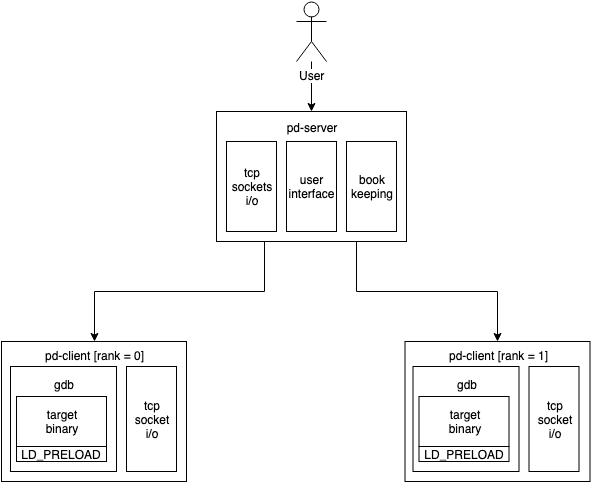
\includegraphics[width=\textwidth]{overview}
  \caption{High level overview of how the parallel debugger works}
  \label{fig:overview}
\end{figure}


\end{document}
